\documentclass[10pt]{beamer}

\usetheme[progressbar=frametitle, titleformat=smallcaps]{metropolis}
\usepackage{appendixnumberbeamer}

\usepackage{booktabs}
\usepackage[scale=2]{ccicons}

\usepackage{pgfplots}
\usepgfplotslibrary{dateplot}

\usepackage{xspace}
\newcommand{\themename}{\textbf{\textsc{metropolis}}\xspace}

\newcommand{\nuc}[2]{${}^{#1}\textrm{#2}$}
\newcommand{\mnuc}[2]{{}^{#1}\textrm{#2}}
\newcommand{\react}[4]{$#1(#2,#3)#4$}
\newcommand{\mreact}[4]{#1(#2,#3)#4}
\newcommand{\alpa}{\react{\mnuc{27}{Al}}{\textrm{p}}{\alpha}{\mnuc{24}{Mg}}}
\newcommand{\nag}{\react{\mnuc{14}{N}}{\alpha}{\gamma}{\mnuc{18}{F}}}
\newcommand{\squared}{${}^{2}$}

\title{
    Verification of Recoil Separator Properties Through Reaction Measurements
}
\subtitle{}
% \date{\today}
\date{November 9, 2018}
\author{Michael T Moran}
\institute{University of Notre Dame}
% \titlegraphic{\hfill\includegraphics[height=1.5cm]{logo.pdf}}

\begin{document}

\maketitle

% \begin{frame}[fragile]{Table of Contents}
%   \setbeamertemplate{section in toc}[sections numbered]
%   \tableofcontents[hideallsubsections]
% \end{frame}

\section{Introduction}

\begin{frame}[fragile]{Capture Reactions}

    Primary burning processes for energy production depend on the
    properties of the star (mass, temperature, enrichment, life cycle
    stage, etc.)

    Hydrogen burning:
    \begin{itemize}
        \item low mass: $pp$-chains
        \item massive stars: CNO, NeNa, and MgAl cycles
    \end{itemize}

    Helium burning:
    \begin{itemize}
        \item Triple-$\alpha$ process
        \item \react{\mnuc{12}{C}}{\alpha}{\gamma}{\mnuc{16}{O}}
            determines C/O ratio
        \item primary sources of neutrons for $s$-process are
            \react{\mnuc{13}{C}}{\alpha}{\rm n}{\mnuc{16}{O}} and
            \react{\mnuc{22}{Ne}}{\alpha}{\rm n}{\mnuc{25}{Mg}} (AGB
            stars)
        \item breakout reactions from cyclic H burning (e.g.
            \react{\mnuc{14}{N}}{\alpha}{\gamma}{\mnuc{18}{F}})
    \end{itemize}

\end{frame}

% \begin{frame}[fragile]{Hydrogen Burning}

%     \begin{figure}
%         \includegraphics[width=0.95\textwidth]%
%             {figures/cno_nena_mgal.png}
%     \end{figure}

% \end{frame}

\begin{frame}[fragile]{Radiative Capture}

    Reactions like $({\rm p}, \gamma)$ and $(\alpha,\gamma)$

    Detecting the $\gamma$ can be difficult due to:
    \begin{itemize}
        \item large background count rates
        \item low count rates
        \item HPGe detector efficiency
    \end{itemize}

    Studied focused primarily on resonances to reduce the effect of
    these problems

\end{frame}

\begin{frame}[fragile]{Inverse Kinematics}

    We can instead detect the heavy recoil particle
    \begin{itemize}
        \item perform the reaction in inverse kinematics
            \react{a}{A}{B}{\gamma}
        \item heavy projectile impinges on light target, heavy recoil
            escapes the target
        \item produced recoil leaves the target and detected by
            high-efficiency detector
    \end{itemize}

    Incident beam also passes through the light target, so we need to
    stop this beam from reaching our detector

\end{frame}

\section{Recoil Separation}

\begin{frame}[fragile]{St.\ George}

    \vspace{1.5em}
    \begin{figure}
        \includegraphics[width=0.95\textwidth]%
            {figures/stg.png}
    \end{figure}

    \tiny{Couder \textit{et al.}, 2008}  % check if this looks OK

\end{frame}

\begin{frame}[fragile]{Magnetic and Electric Rigidities}

    Elements within St.\ George are tuned for the $B\rho$ and $E\rho$ of
    the recoil particle
    \[
        \begin{split}
            B\rho = \frac{\sqrt{2mT}}{q}
        \end{split}
        \quad\quad
        \begin{split}
            E\rho = \frac{2T}{q}
        \end{split}
    \]

    Design limits: $0.1 \leq B\rho \leq 0.45$~Tm and $E\rho \leq 5.7$~MV

\end{frame}

\begin{frame}[fragile]{Particle Selection}

    We can uniquely identify particles by their mass, charge and energy:

    \begin{alertblock}{Magnetic Selection}
        % \[
        %     \frac{m}{q} = \frac{B\rho}{2}\left(\frac{T}{q}\right)^{-1}
        % \]
        selects a single momentum: $p = q \cdot B\rho$
    \end{alertblock}
    \begin{alertblock}{Electric Selection}
        % \[
        %     \frac{T}{q} = \frac{E\rho}{2}
        % \]
        selects a single energy: $T = q/2 \cdot E\rho$
    \end{alertblock}
    \begin{alertblock}{Wien Filter Selection}
        % \[
        %     \frac{m}{q} = \frac{2}{v^2} \frac{T}{q}
        % \]
        selects a single velocity: $v = E/B$
    \end{alertblock}

    % $B\rho$ and $E\rho$ are the magnetic and electric rigidities of the
    % particle in question

\end{frame}

\begin{frame}[fragile]{Particle Selection}

    \vspace{1em}
    Any two of the three possibilities may be combined to uniquely
    identify a particle

    \begin{figure}
        \includegraphics[width=0.75\textwidth]%
            {figures/particle_selection_by_field.png}
    \end{figure}

\end{frame}

\begin{frame}[fragile]{Angular and Energy Acceptance}

    Recoils can only be transported within defined parameter bounds
    \[
        \begin{split}
            \Delta E/E = \pm7.5\,\%
        \end{split}
        \quad\quad
        \begin{split}
            \Delta\theta = \pm40\,\text{mrad}
        \end{split}
    \]

    These bounds must hold for all possible $E\rho$ and $B\rho$

\end{frame}

\begin{frame}[fragile]{Importance of Acceptances}

    Verifying the acceptances across a wide range of $B\rho$ and $E\rho$
    is required in order to eliminate it as a potential source of error

    Ensures that all of the produced recoils and none of the incident
    beam particles for a given reaction reach the detector plane
    \begin{itemize}
        \item produced recoils can be extremely rare (1 for every
            $10^{15}$ beam particles)
    \end{itemize}

    Once acceptances have been verified for enough $B\rho$ and $E\rho$
    possibilities, scaling the electromagnetic elements to other
    rigidity values should retain the acceptance properties

\end{frame}

\section{Commissioning}

\begin{frame}[fragile]{Types of Commissioning}

    The goal is for 100\,\% of the produced recoils to make it to the
    final detector plane

    Can divide commissioning between three possible cases:

    \begin{alertblock}{Energy}<2->%<1-| alert@4> for highlighting
        change the particle energy without interfering with the other
        quantities
    \end{alertblock}
    \begin{alertblock}{Angular}<3->
        change the deflection of the particle at the target location
    \end{alertblock}
    \begin{alertblock}{Joint}<4->
        adjust both at the same time
    \end{alertblock}

\end{frame}

% \begin{frame}[fragile]{Goal of Commissioning}

%     For a properly-tuned separator, 100\,\% of the recoil particles will
%     be transmitted to the final detector plane
%     \begin{itemize}
%         \item Can measure current at the target and detector location
%         \item Can use a particle detector (if current low enough)
%     \end{itemize}

%     Will be true for particles within the designed angular and energy
%     acceptance windows for a single tune of the separator

% \end{frame}

\begin{frame}[fragile]{Energy Acceptance}

    For a particle beam with a given $B\rho$ and $E\rho$:

    \begin{itemize}
        \item Tune the test beam to a given energy, and
            tune St.\ George for that energy
        \item Verify 100\,\% transmission, adjust the tune
            if necessary
        \item Adjust the beam energy within the energy
            acceptance bounds and measure transmission
        \item Adjust the tune if necessary to have 100\,\%
            transmission for all possible energy changes within the
            acceptance bounds
    \end{itemize}

\end{frame}

\begin{frame}[fragile]{Energy Acceptance}

    \vspace{0.5em}
    Energy acceptance completed for a subset of $B\rho$ and $E\rho$
    test particles (100\,\% transmission found through current
    measurements)

    \begin{figure}
        \includegraphics[width=0.75\textwidth]%
            {figures/rigidity_phase_space.png}
    \end{figure}

    \tiny{Adapted from Meisel, \textbf{Moran}, \textit{et al.}, 2017}

\end{frame}

\begin{frame}[fragile]{Angular Acceptance}

    For a particle beam with a given $B\rho$ and $E\rho$:

    \begin{itemize}
        \item Tune the test beam to a given energy, and
            tune St.\ George for that energy
        \item Verify 100\,\% transmission, adjust the tune
            if necessary
        \item ``Deflect'' the beam at the target location
            within the acceptance bounds (horizontally and vertically)
        \item Adjust the tune if necessary to have 100\,\%
            transmission for all possible angular changes within the
            acceptance bounds
    \end{itemize}

\end{frame}

\begin{frame}[fragile]{Joint Acceptance}

    All experiments will have an angular and energy spread, so must
    confirm that the acceptances can be achieved at the same time
    % \begin{itemize}
    %     \item Following the previous procedures, but interwoven, would
    %         take too long for each point
    % \end{itemize}

    Can use a degrader foil to create an angular and energy spread at
    the same time
    \begin{itemize}
        \item New central energy based on energy loss
        \item Target material and thickness extremely important to
            understand well
        \item ``Fuzziness'' of beam spot may still make it difficult
            to tune
    \end{itemize}

\end{frame}

\section{Reaction Measurements}

\begin{frame}[fragile]{Justification for Reaction Measurements}

    Joint acceptance measurements are costly to cover all of the
    possibilities

    Reactions can be used to ``bootstrap'' the process
    \begin{itemize}
        \item Reactions have a known cross section, angular and energy
            spread, etc.
        \item If all of the expected produced recoils reach the
            detector, the separator is performing optimally
    \end{itemize}

\end{frame}

\begin{frame}[fragile]{The \alpa{} Reaction}

    \vspace{1.5em}
    \begin{figure}
        \includegraphics[width=0.65\textwidth]%
            {figures/reaction_energy_diagram.png}
    \end{figure}

\end{frame}

\begin{frame}[fragile]{The \alpa{} Reaction}

    \vspace{0.5em}
    Cross section is well-known, reducing it as an uncertainty in the
    measurements

    \begin{figure}
        \includegraphics[width=0.75\textwidth]%
            {figures/zero_degree_pa0.png}
    \end{figure}

    \tiny{Courtesy of R.\ J.\ deBoer, 2017}

\end{frame}

\begin{frame}[fragile]{Alternate Tune}

    Since the last segment of St.\ George has not been fully
    commissioned (full angular acceptance not yet verified), we can use
    the focal plane after the Wien filter to perform cross section
    measurements

    For $({\rm p},\alpha)$ reactions, the expected beam suppression is
    sufficient to reject the high-intensity incident beam

    The beam spot at this focal plane needs to be adjusted to direct the
    reaction products to the detector

\end{frame}

\begin{frame}[fragile]{Alternate Tune}

    \vspace{1.5em}
    Determined expected field strengths using \verb+COSY+ and verified
    with direct particle transport before the experiment

    \begin{figure}
        \includegraphics[width=0.75\textwidth]%
            {figures/optimal_tune_x.png}<1>
        \includegraphics[width=0.75\textwidth]%
            {figures/optimal_tune_y.png}<2>
    \end{figure}

\end{frame}

\begin{frame}[fragile]{Angular Acceptance Measurement}

    The reaction \alpa{} emits the $\alpha$ particles within an
    isotropic angular distribution
    \begin{itemize}
        \item target cup restricts us to $\approx 40$~mrad acceptance
        \item we will attempt to transport all $\alpha$ particles to the detector
    \end{itemize}

    Tuning the beginning of the separator to transport the particles to
    the Wien filter focal plane is an alternative to a full angular
    acceptance measurement

    Ability to fine-tune and have confidence in the properties of the
    separator are required

\end{frame}

\begin{frame}[fragile]{Acceptance Measurements}

    % \vspace{1.5em}
    \begin{figure}
        \includegraphics[width=0.85\textwidth]%
            {figures/acceptance_uncertainty.png}
    \end{figure}

\end{frame}

\begin{frame}[fragile]{Acceptance Uncertainty}

    We can attribute the uncertainty at each measurement to the
    underlying variables within our control: energy, current, time, and
    target thickness
    \begin{itemize}
        \item On-resonance: dominated by current uncertainty
        \item Below resonance: dominated by energy uncertainty
        \item Attribution through a hybrid Monte Carlo/Bayesian
            approach
    \end{itemize}

    Final irreducible uncertainty cannot be avoided, but controllable
    uncertainty can be minimized

\end{frame}

% \begin{frame}[fragile]{Acceptance Measurements}

%     On-resonance, we are consistent with a $\Delta\theta = 40$~mrad
%     acceptance

%     Off-resonance, we have larger uncertainty and are limited by a lack
%     of diagnostics

%     Systematic trends around each resonance can be due to non-uniform
%     angular acceptance (seen during preliminary tests)

% \end{frame}

\section{Future Directions}

\begin{frame}[fragile]{Experimental Outcome}

    St.\ George has been shown to have the following acceptances:
    \begin{itemize}
        \item $\Delta E/E \geq \pm 7.5$\,\%
        \item $\Delta E/E = \pm 3$\,\% and $\Delta\theta = \pm 40$~mrad
            (to WF)
    \end{itemize}

    Preliminary beam reduction measurements on the order of $10^{12}$

    Separation properties and beam currents are suitable for low-energy
    and off-resonance cross section measurements

\end{frame}

\begin{frame}[fragile]{The Future of St.\ George}

    \begin{itemize}
        \item St.\ George can be used for a restricted subset of
            experiments
        \item Ability to fine-tune the separator and verify its
            properties over a range of $B\rho$ and $E\rho$ values
            essential for future experiments
        \item Diagnostic equipment and procedures developed to be
            applied to future separators (SECAR)
        \item Final parts of the St.\ George system (HIPPO supersonic
            jet gas target, full detector system, additional
            diagnostics, etc) will unlock the full range of experimental
            work
    \end{itemize}

\end{frame}

\maketitle

\appendix

% potential slides:
% - tables showing the uncertainty values
% - detailed run plan
% - astrophysics support? PP, CNO, etc?
% - R-matrix (plus extra details)
% - STG planned reactions
% - detector spectra

\begin{frame}[fragile]{95\,\% Contributions}  % build out backup slides

    \begin{figure}
        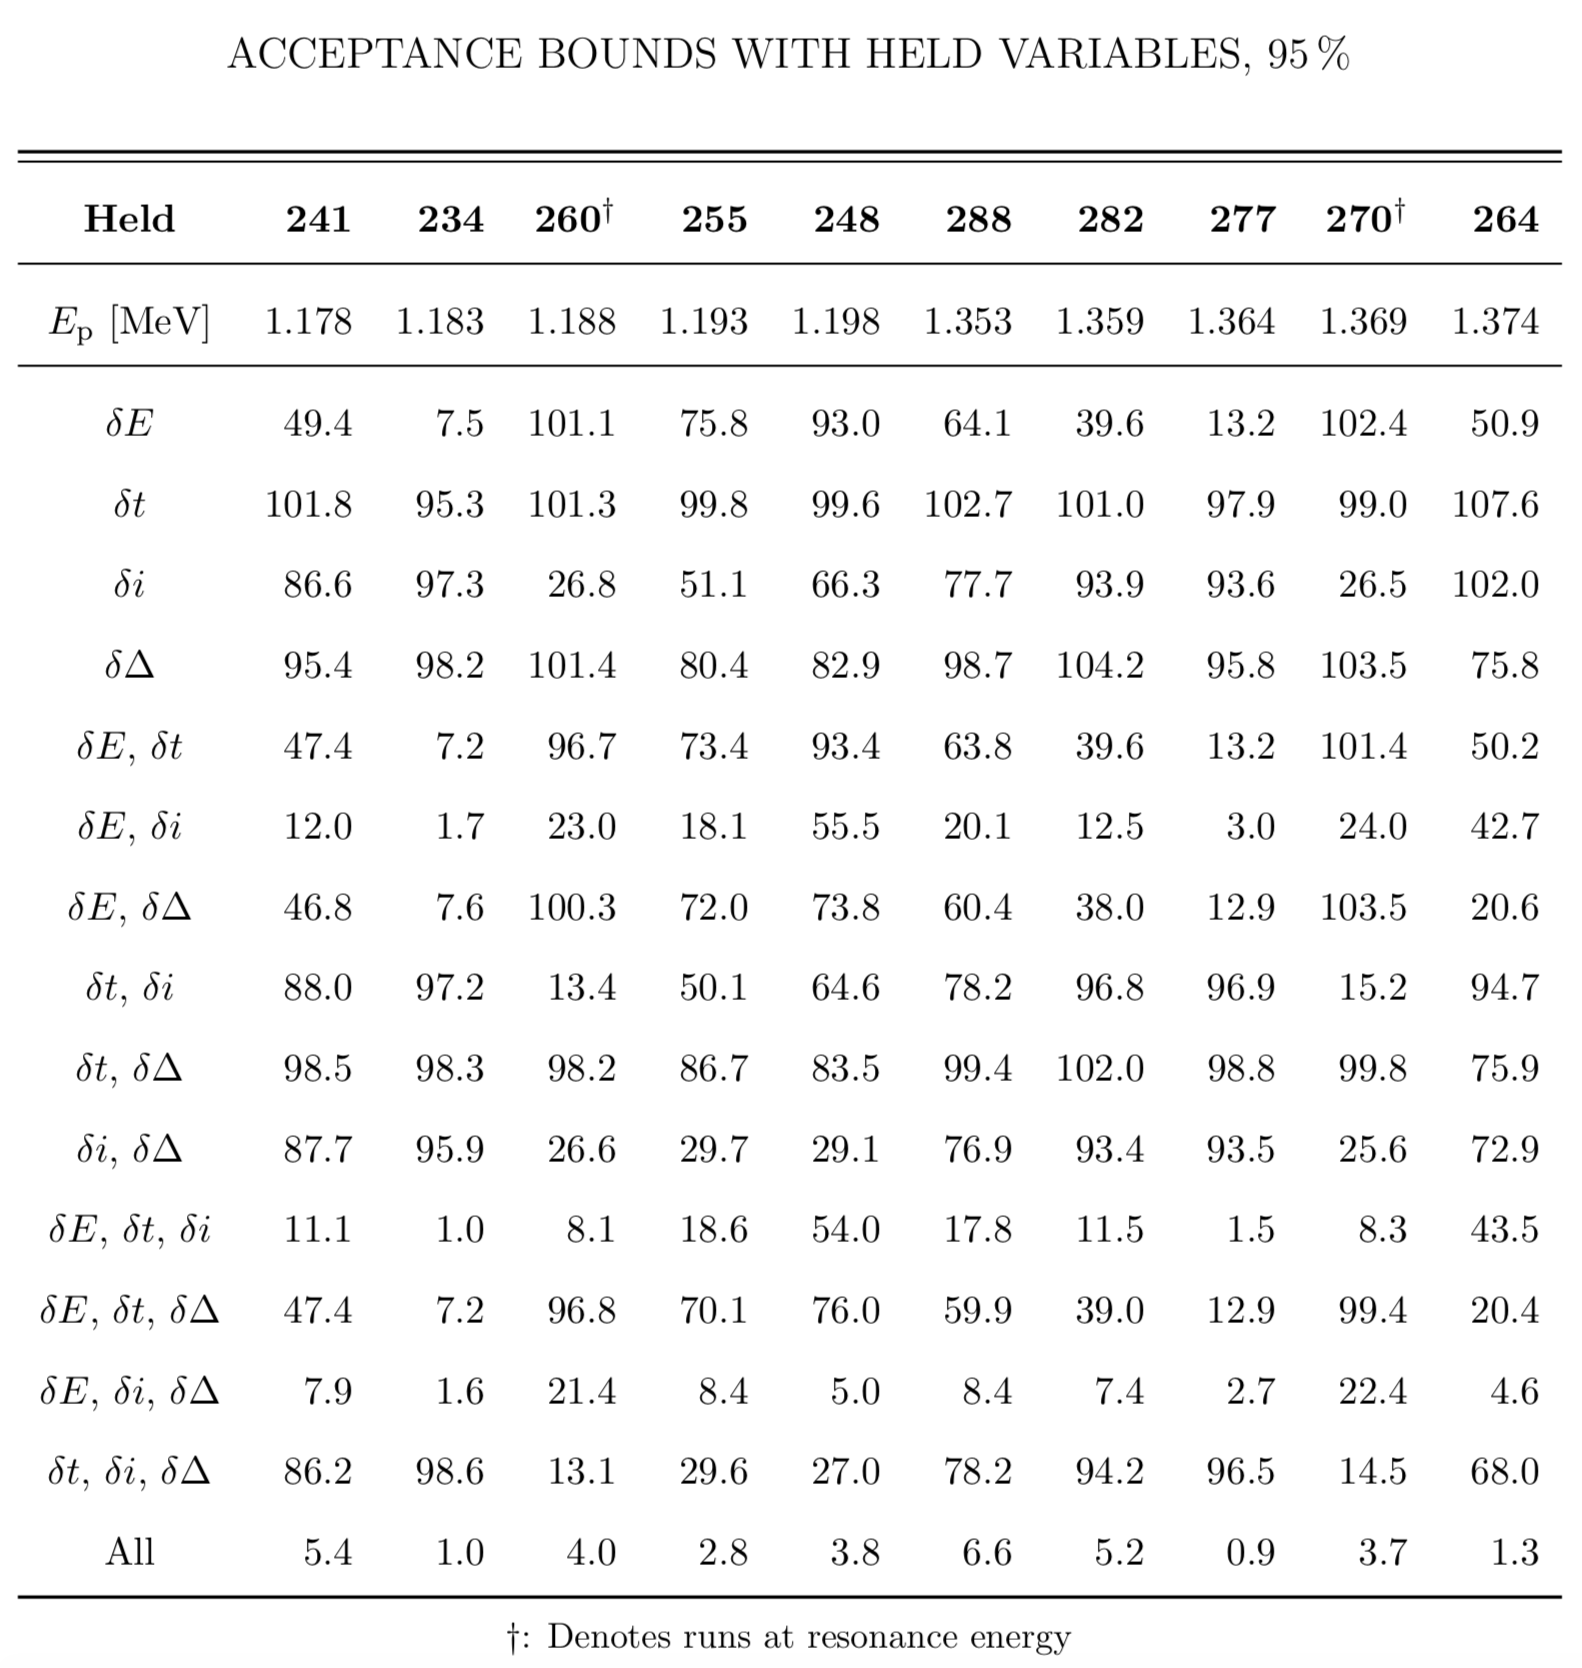
\includegraphics[width=0.7\textwidth]{figures/table_95.png}
    \end{figure}

\end{frame}

\begin{frame}[fragile]{Initial Test Reactions}

    \begin{figure}
        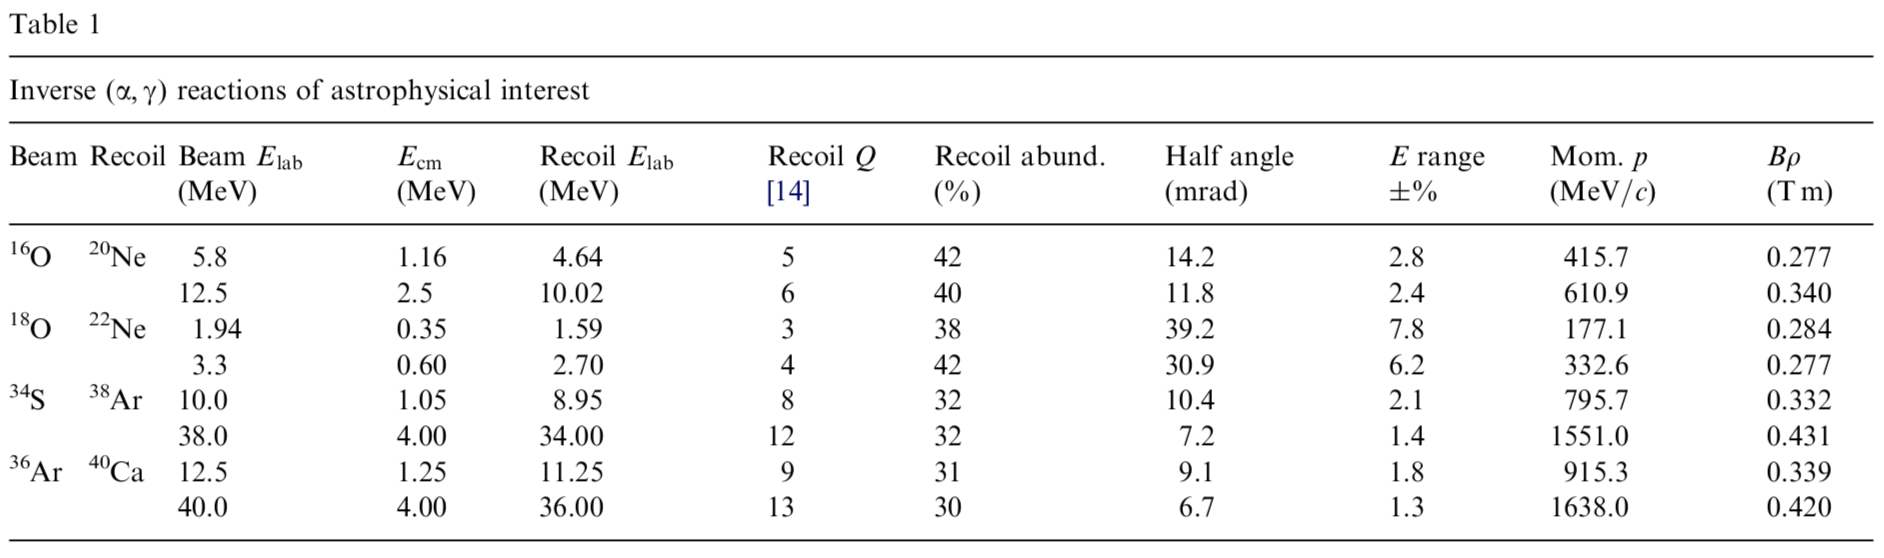
\includegraphics[width=\textwidth]{figures/stg_reactions.png}
    \end{figure}

\end{frame}

% \begin{frame}[allowframebreaks]{References}
%   \bibliography{defense}
%   \bibliographystyle{abbrv}
% \end{frame}

\end{document}
